\documentclass[12pt]{report}
\usepackage[utf8]{inputenc}
\usepackage{graphicx}
\usepackage[en-US]{datetime2}
\usepackage{fancyhdr}
\usepackage{tabularx}
\usepackage{siunitx}
\usepackage{graphicx}
\usepackage{float}
\usepackage{multirow}
\usepackage{multicol}
\usepackage{enumitem,amssymb}
\usepackage{algorithm}
\usepackage{subfig}
\usepackage{biblatex}
\addbibresource{references.bib}
\setlength\headheight{15pt}

\usepackage{nicefrac}
\usepackage{amsthm,bm}
\usepackage[percent]{overpic}
\usepackage{wrapfig}
\usepackage{amsmath}

\usepackage{verbatim}
\usepackage{booktabs}
\usepackage{mathtools}
\usepackage[normalem]{ulem}
\usepackage{array}
\usepackage{cuted}

% \usepackage{etoolbox}% http://ctan.org/pkg/etoolbox
% \makeatletter
% \patchcmd{\@makechapterhead}{\vspace*{50\p@}}{}{}{}% Removes space above \chapter head
% \patchcmd{\@makeschapterhead}{\vspace*{50\p@}}{}{}{}% Removes space above \chapter* head
% \makeatother

% %%%%%% line numbers:
% \usepackage[right]{lineno}
% \usepackage{blindtext,color}
% \renewcommand\linenumberfont{\normalfont\scriptsize\color{red}}
% \linenumbers

\newcommand{\Li}{\textbf{(i)}\ }
\newcommand{\Lii}{\textbf{(ii)}\ }
\newcommand{\Liii}{\textbf{(iii)}\ }
\newcommand{\Liv}{\textbf{(iv)}\ }
\newcommand{\Lv}{\textbf{(v)}\ }
\newcommand{\Lvi}{\textbf{(vi)}\ }


\newlist{todolist}{itemize}{2}
\setlist[todolist]{label=$\square$}
\usepackage{pifont}
\newcommand{\cmark}{\ding{51}}%
\newcommand{\xmark}{\ding{55}}%
\newcommand{\done}{\rlap{$\square$}{\raisebox{2pt}{\large\hspace{1pt}\cmark}}\hspace{-2.5pt}}
\newcommand{\wontfix}{\rlap{$\square$}{\large\hspace{1pt}\xmark}}
\pagestyle{fancy}
\graphicspath{ {images/} }

\newcommand{\ft}{4,835 }
\newcommand{\hn}{DualGraph}
\usepackage{amsmath}

\title{
    {Harnessing Simulated Datasets with Graphs}\\
    {\large Thesis Dissertation Proposal}\\
    {\large Columbia University}\\
}
\author{Henrique Teles Maia}
\date{\today}

\begin{document}

\maketitle

\begin{abstract}
% Data-driven techniques are ubiquitous across engineering disciplines.
% In this proposal, we discuss how to pair simulated data with graph algorithms 
% in order to control the expansion of states that naturally appear when collecting observations.
Physically accurate simulations enable the generation of 
limitless data from within meticulously crafted environments. 
Digital sandboxes allow for collecting observations at-will and in arbitrary scenarios.
This is particularly useful given the ubiquity of data-driven techniques across engineering disciplines.
These are systems which inform behavior from aggregating over available samples.
% Paired together with statistical methods, the partnership of synthetic data with data-driven models
Paired together with statistical methods, the ability to synthesize endless data
promises to make approaches that benefit from datasets all the more robust and desirable. 
However, if not careful, pipelines that naively aim to measure virtual scenarios
can easily be overwhelmed by trying to sample an infinite set of available configurations.
% However the ability to measure virtual scenarios in turn extends the procured samples
% into a dangerously infinite set of configurations, 
% and can quickly overwhelm the feature space of a system.
Variations observed across multiple dimensions can quickly lead to a daunting expansion of states,
which must be processed and solved.
Therefore we propose to wield graphs in order to instill structure over captured data,
and curb the growth of variables.
The graphs we introduce serve to enforce consistency, localize operators, 
and crucially factor out any combinatorial explosion of states. 
We demonstrate the effectiveness of this methodology in three distinct areas, 
each offering their own challenges and practical constraints. 
Namely, we observe state-of-the-art contributions in design for additive manufacturing, 
side-channel security threats, and large-scale physics based contact simulations, 
that are achieved solely by harnessing simulated datasets with graph algorithms.
\end{abstract}

\setcounter{secnumdepth}{1}
\setcounter{tocdepth}{1}
\tableofcontents

\chapter{Introduction}\label{intro}
\vspace{-9mm}
% \section{Problem Statement}
% In this proposal we 
The objective of the research described in this dissertation is to
channel the efforts required to leverage 
large handcrafted datasets by
structuring the observations as graphs.
% traversing over the observations via graphs. 
% We particularly focus on data collected from simulated and controlled environments, 
% since these provide for physically accurate and realistic models of behavior. 
Most data-driven techniques place the burden of sorting and sifting through
features in their data to downstream optimization techniques.
However, virtual measurements make it easy to capture an abundance of labeled entries
in diverse and arbitrary states.
Adequately sampling these configurations leads to an exponential and combinatorial growth 
of the dataset that cause difficulties to most numerical methods.
Is it therefore necessary to first shape and funnel features drawn from large quantities of complex, 
high dimensional, and interdependent variables.

We find graphs are generally suited to assembling dependencies that are easier to operate over.
Graphs map domain expertise into assumptions, 
constraints, and connections that can be generalized over the data.
This added consistency complements the dataset 
by assisting with the combinatorics of the observed samples.
Therefore, through careful structuring of the data into graph-like structures, 
we can safely expose our algorithms to varied conditions with an understanding of how the system 
will perform and scale.

The benefit of such an approach is the ability to tackle real and physical constraints via
an unconstrained dataset of hand-crafted and curated observations. 
Systems that utilize graph treatment over instances of the data are flexible.
Such methods can adapt to new situations, without additional computational burden, 
by simply adjusting the data used to drive the pipeline as new data becomes available. 
We particularly focus on data collected from simulated and controlled environments, 
since these provide for physically accurate and realistic models of behavior. 
We present a methodology that outlines how to cast synthetic datasets into a structure 
whose processing guarantees simpler frameworks and ultimately more robust applications. 


% We validate this methodology as it applies to computer vision tasks on real world 3D printed
% objects (Ch.~\ref{layercodes}), side channel extraction of neural network topologies from
% active GPUs (Ch.~\ref{snoop}), and lastly efficient strand contact simulation (Ch.~\ref{plan}).
% We show that compared to alternative methods this 
% handling of data driven models outperforms in terms of robustness and quality guarantees.

\section{Methodology}\label{sec:method}
% Leverage simulation to tackle real physical constraints via hand-crafted dataset. 
% Where is this useful/used/necessary?
% Codify the process that a body of work has been trying to do
% Introduce a methodology that frames the survey of existing works who try to tackle similar issues
% How is this already used (perhaps not in a nicely synthesized way as your thesis will provide)
% How did I use it in my papers
% Why is simulated data useful/better than real world?
% Sim2real \& Real2Sim
% Compensate for uncertainties with simulated where we know everything, adding fidelity from simulation to the real world measurements


% \subsection{Motivation}

The goal of many researchers to achieve and model realistic behavior. 
We propose a methodology for collecting and utilizing large sets 
of simulated data to inform realistic models of behavior in conjunction with graph algorithms. 
Simulated and synthetic examples are not limited like their real world annotated counterparts.
Digital observations are collected at low cost, can be automated,
and permit studying of arbitrary scenarios and interactions.
Their exploratory discretion is not without fault however,
as this added freedom also adds both complexity and degrees of freedom to the measurements taken.
In turn, generalized patterns must be formulated across the dataset to reduce
this combinatorial expansion of variables.
Graphs restrain the space of features considered by
focusing computational operations on nodes and edges.
Categorizing data into these primitives also simplifies the relationships between values 
by explicitly laying out dependencies.
Therefore, we believe that graphs are specifically positioned to assist with
data driven approaches that have exploded in popularity over the past decade. 

Our methodology is as follows:
\begin{enumerate}
    \item Generate a specialized dataset from synthetic data to assist an objective
    \item Identify combinatorial challenges and inter-sample patterns to factor
    \item Overlay a graph to instill structure and manage the spectrum of states
    \item Leverage graph algorithms to operate on the data via this distilled lens
\end{enumerate}

\subsection{Contributions}\label{sec:contributions}
We investigate challenges receptive to digitally acquired datasets 
from applications in diverse problem areas.
We validate this methodology as it applies to computer vision tasks on real world 3D printed
objects, side channel extraction of neural network topologies from
active GPUs, and lastly efficient strand contact simulation.
We show not only that this approach is broadly applicable, 
but that systems that partner data driven models with graph algorithms
outperform existing methods in terms of robustness and quality guarantees.

% The contributions are as follows:
% \begin{enumerate}
%     \item 
%     \item 
%     \item 
% \end{enumerate}

\section{Roadmap}\label{sec:roadmap}
The product of this dissertation will be a study of the benefits to marrying graph structures with
simulated data collection in modeling various behaviors. 
Our proposed assessment consists of three studies:
\begin{enumerate}
    \item \textbf{LayerCodes} (Ch.~\ref{layercodes}) We observe how simulated proxies can assist with the design
    of physical tags that embedd information in additive manufactured geometries.
    The resulting approach relies on graph structures to produce a robust tag given the complex interplay
    of unconstrained geometries present in the dataset.
    \item \textbf{Neural Snooping} (Ch.~\ref{snoop}) Diverse network architectures are distilled into graphs
    for extraction and reconstruction through electro-magnetic side channel attacks. Through carefully
    curated synthetic datasets we are able to recover large and deep black-box designs to great fidelity.
    \item \textbf{Data-Driven Hair Contact} (Ch.~\ref{plan}) We propose to apply our methodology against 
    the inefficiencies of contact resolution in large scale elastic-rod interactions 
    by training Graph Neural Networks on simulation data.
\end{enumerate}
Taken together, these evaluations survey the range of applications that stand to benefit by combining powerful graph techniques with limitless synthetic data points.

\chapter{Related Work}\label{related}

Here we overview recent advances in data-driven techniques broken into several general areas:
\begin{enumerate}
    \item \textbf{Sim-2-Real \& Real-2-Sim}: Bridging 
    % the gap between 
    real world measurements and applications with digital models and representations. 
    \item \textbf{Data-Driven Techniques}: Leveraging statistical analysis over collected databases to inform heuristics and algorithms.  
    \item \textbf{Graph Algorithms}: The involvement of graphs, trees, and more contemporary techniques to instill structure over data within algorithms.
\end{enumerate}

\paragraph{Sim-2-Real \& Real-2-Sim}\label{sec:rel_real2sim}

The task of Sim-to-Real, and conversely Real-to-Sim, 
transfer is one shared by many application areas.
Simulations provide controlled environments for 
gathering observations and experimentation at low cost.
However, their validity is highly dependent 
on an accurate representation of the real world.
% Therefore, large research efforts are made to develop
% faithful models, careful measurements, and robust algorithms
% in order to allow transfer between digital and physical modalities.

Simulated models are often intended to be used in the real world.
Applications in robotics design practice in digital sandboxes before entering 
reality~\cite{kappler2015leveraging,romano2011human,varley2017shapecompletion_iros}.
Similarly, techniques in computer vision are often tailored to 
interpret real images and align them with software
interactions~\cite{Epstein_2020_CVPR,jo2016shutter,CAVE_0352}.
The gap between simulation and reality must also be faced when preparing security applications,
as software and hardware considerations must be taken into account to contend with
digital and physical attacks ~\cite{batina2019csi,hu2020deepsniffer,maia2021hear}.

On the other hand, it is often fruitful to guide the development 
of a digital technique with real world measurements. 
Principled values facilitate parameter tuning in the case of physics-based simulations,
which combine mechanical and physical equations to produce dynamic 
behavior~\cite{chen2021boombox,Fei2017wetHair,adonis14}.
Careful understanding and measurement of the real world can also inform design.
Such is the case most prominently when manufacturing features that depend on physical interactions,
as in the fields of physical information embedding~\cite{ding2017air,Li:2016:acoustic_voxels,Maia:2019}
and digital design for fabrication~\cite{Schulz2017cad,Schulz2017robogami,shulz2018trade}.

\vspace{-2mm}
\paragraph{Data-Driven Techniques}\label{sec:rel_data}
Curated datasets provide alternatives when precise behavioral models are unavailable or expensive.
Often these measurements provide an input-output pair collected by labeling real world data,
as is often the case with image based datasets~\cite{deng2009imagenet,deng2012mnist}.
These datasets feature practical scenarios in the wild, 
but can often times be laborious or subjective to label.
Data-driven techniques can also benefit from synthetic collections,
such as those comprised of 3D objects or paths~\cite{calli2015ycb,goldfeder2009columbia,Thingi10K},
as is often of interest to those in robotics. 
Regardless of their form, these datasets describe aggregate behavior that
can be used to statistically dictate algorithms.

Data-driven models approximate complexity in a variety of ways.
Model-reduction techniques couple datasets with simplified or scaled behavioral models.
These include methods that make simplifying assumptions about dynamic 
behavior~\cite{Fei2018wetcloth,Fei2017wetHair}, 
or project degrees of freedom into a lower dimensional---and thereby easier to solve---space
\cite{goldfeder2011data,xu2015modelreduc}.
Machine learning approaches pair neural networks with data to great effect.
By linking results to data features through gradient descent and back-propagation,
applications in
vision~\cite{he2016vision},
security~\cite{xu2017security},
natural language processing~\cite{teufl2010nlp}, 
and robotics~\cite{kober2013robotics},
all stand to benefit from larger datasets when possible, 
and have been shown to work with both synthetic and real data.

\vspace{-2mm}
\paragraph{Graph Algorithms}\label{sec:rel_graph}
% \subsubsection{Traditional}
Mathematical graph theory extends into computer science by way of graph data types
and traversal algorithms.
These approaches define rules over collections of nodes and edges, attributing each with 
specific properties and relationships to one 
another~\cite{harris2009combinatorics, papadimitriou1998combinatorial}.
This gives structure abstractly to data formulated in such primitives, 
e.g. limiting data in a graph node to only interact with incident edges or neighboring nodes.
% \subsubsection{Graph Neural Networks}

Recently these approaches have been combined with machine learning techniques to
directly benefit from datasets. 
The result is the introduction of Graph (Neural) Networks who host embeddings
on nodes and edges of a graph that can influence one another
through neural-graph hybrid 
operations~\cite{battaglia2018graphnetssummary,pfaff2021learning,sanchezgonzalez2020learning};
and profit from both data-driven and graph techniques. 

\chapter{LayerCodes}\label{layercodes}

% \begin{figure}[h]
%     \centering
%     \includegraphics[width=0.99\textwidth]{figs/teaser.pdf}
%     \caption{
%     \textbf{LayerCode tags} are deployed in 3D printed objects 
%     through two-color printing (a), variable
%         layer heights (d), and near-infrared steganography (g).
%         In the first case (a), the LayerCode tag is visible;
%         in the second (d), the tag is less visible; and in the third (g)
%         it is completely invisible, but still machine-readable.
%         Just like reading a barcode,
%         we capture an image of each object,
%         and our decoding algorithm processes the image to create a decoding
%         graph (b, e, h), from which a linear barcode (and thus the corresponding
%         bit string) is recovered (c, f, i).
%         }
%     \label{fig:layercode_teaser}
% \end{figure}
\vspace{-9mm}
With the ongoing advance of personal and customized fabrication techniques, 
the capability to embed information in physical objects has become both more crucial and challenging. 
Traditionally optical barcodes serve as the indispensable link that bridges
physical artifacts to modern digital systems.
However, barcodes rely on constrained industrial designs that mandate flat and smooth geometries.
In this work, we rethink barcodes in the context of additive manufacturing,
popularly known as 3D printing. 3D printing offers a quick way of making 
customized, complex shaped objects.
Unlike a mass-produced product which by design has a reserved flat surface region
to host barcodes, 3D printed shapes are often complex and curved: 
thin features, slender threads, and holes are not uncommon.
As a result, the traditional barcodes cannot be placed or printed on such objects.

% Granted the ability to simulate renderings of any potential solution, 
We apply our methodology to improve the optical tagging of custom 3D shapes.
We motivate our design by generating a dataset of \ft printable shapes, 
along with image renderings of our objects from various views,
that allows us to experiment and preview challenges specific to customized geometries.
We study this dataset to identify local invariants common to all shapes,
regardless of holes or intricate features.
These local properties are extracted from renderings of tagged objects and used to construct a graph,
which abstracts out spatial complexities, allowing all custom shapes to be treated uniformly.
Traversing this graph we achieve a robust in-plain-sight algorithm 
that enables the 3D printing layers to carry information without altering the object's geometry.
We name our tagging scheme \emph{LayerCode}, and demonstrate how a carefully designed pattern 
may be directly embedded in objects as a deliberate byproduct of the 3D printing process. 
We show that LayerCodes work across various types of 3D printers, 
and succeed on complex, nontrivial shapes, on which previous tagging mechanisms all fail. 

% decoding algorithm that is applicable
% to tags physically deployed across various types of 3D printers.
% % including Fused Deposition Modeling printers as well as Stereolithography based printers. 
% The result is a tag that works on complex, nontrivial shapes, 
% on which all previous tagging mechanisms may fail. 

% % Conceptually the LayerCode is inspired by the structural 
% % resemblance between the parallel two-tone bars 
% % of the standard barcode and the universal layer-by-layer approach of 3D printing. 
% However, the success of its design is tied to
% Our efforts result in 
% an in-plain-sight encoding algorithm 
% that enables the 3D printing layers to carry information without altering the object's geometry. 
% % This process is complemented by a decoding graph algorithm 
% % that reads the LayerCode tag of a physical object from a photo. 
% % LayerCode tags are physically deployed across various types of 3D printers, 
% % including Fused Deposition Modeling printers as well as Stereolithography based printers. 
% % Each offers its own advantages and trade-offs, 
% % and all rely on the same underlying graph concepts that were developed on simulated examples. 
% % Notably, in order to evaluate LayerCode implementations thoroughly and efficiently, 
% % we stress test it with a large dataset of complex shapes using virtual rendering. 
% % Among \ft tested shapes, our proposed tagging approach successfully 
% % encodes and decodes on more than 99\% of the shapes. 
% The result is a tag that works on complex, nontrivial shapes, 
% on which all previous tagging mechanisms may fail. 

% We introduce/present
% We explore LayerCode, a tagging scheme that embeds a carefully designed barcode pattern in 
% 3D printed objects as a deliberate byproduct of the 3D printing process. 


\paragraph{Objective}
% \emph{LayerCode} 
LayerCodes aims to bring the concept of optical barcodes into 3D printed objects, 
especially those with curved shapes and fine structures.
Our key idea is inspired by a structural resemblance between optical barcodes
and 3D printed objects: essential in a barcode are its two-tone bars
arranged in parallel; universal in all 3D printed objects are the printing
layers introduced in a parallel fashion. 
In fact, virtually all additive manufacturing uses a 
layer-by-layer printing process~\cite{LivesuEMLA17,redwood20173d}.
Thus, if we could interleave two categories of layers in a 3D printing process---be 
it through color, texture or otherwise---we 
would be able to embed a tag everywhere in a 3D printed object. 

%  challenges, resolved by algorithmic, dataset, graph
Materializing this idea faces major algorithmic and combinatorial challenges.
Due to an object's complex shape, 
its layering structure may appear curved, disconnected, 
or shadowed when captured by a camera. 
It is difficult to anticipate how these effects will interplay under perspective projection
without first deploying any proposed encodings across a variety of objects.
Moreover, unconstrained printable shape geometries, 
such as those allotted by customized fabrication,
readily combine in a diversity and frequency of patterns 
that can easily overwhelm naive decoding approaches that fail to generalize.
We therefore seek a robust encoding and decoding algorithm 
that embeds information in printing layers and 
later retrieves this information from the images of a conventional camera.

\section{Method}\label{sec:layercode_method}

We address these challenges by introducing a new coding algorithm and 
verifying it through a large dataset of simulated examples.
Unlike the standard barcode that maps every bit to a fixed bar thickness, 
we encode individual bits based on the local change of layer thickness.
We will show that such local changes are invariant 
under different surface orientations and curvatures.
At decoding time, we exploit a key observation 
that each layer spans the entire cross-section of the object. 
This suggests that there exist many image-plane paths along which we can decode. 
The rich set of decoding paths is advantageous,
enabling us to sidestep shadows, highlights, and uncertain image regions.
Together these steps allow us to tag robustly, 
as supported through both simulated and real-world LayerCoded geometries.

\subsection{Encoding}\label{sec:layercode_encode}

% \begin{figure}[t]
%     \centering
%     \vspace{-5mm}
%     \includegraphics[width=0.60\linewidth]{figs/sphere-figure3.pdf}
%     \vspace{-2mm}
%     \caption{\textbf{Distorted thickness.} Layers of equal thickness on a sphere. Curvature and perspective cause layers to appear spatially varying in size.
%     \label{fig:bw_layers}}
%     \vspace{-3mm}
% \end{figure}

The input to our encoding algorithm is a 3D shape, the tag information
represented as a bit string, as well as the printing direction with
respect to the printed object
(i.e., the direction along which 3D printing layers will be grown). 
Unlike other tagging methods, there is no restriction on the 3D printed shape.
We leave the flexibility of choosing a printing direction to the user,
because the printing direction may depend on the specific shape, printing
software, support materials, and perhaps semantic or subjective preferences.
The output of the encoding algorithm is a series of slices along the printing
direction to specify the thickness of each coding layer.

Our key insight comes from noticing the fact that if the coding layers are thin
(relative to the inverse of the surface curvature along the printing direction),
the thickness \emph{ratio} of two consecutive layers measured in a local region
of the image plane is \emph{invariant}. This is because in a small local region,
two nearby coding layers share approximately the same surface tangent plane, and the
projection from the tangent plane to the image plane follows an affine
transformation which preserves the layer thickness ratio.

Using local thickness ratios also favors the decoding step. 
It allows us to sample the thickness
ratio of two layers at many local regions on a captured image, and collectively
estimate a thickness ratio that is robust against imaging noise and artifacts.

\paragraph{Coding scheme}
We propose the following scheme to encode every bit in a bitstring.
A bit ``\textbf{1}'' is encoded if the thickness ratio of two consecutive layers is either
$\nicefrac{1}{M}$ or $M$, where $M$ is a constant larger than 1 that we will
discuss shortly, and a bit ``\textbf{0}'' is represented by a unitary thickness ratio
(i.e., the same thickness).
The representation of a bit string always starts from a layer with a baseline
thickness $h$. The next layer thickness $a_{n+1}$ is either $h$ or $Mh$
according to the current bit $b_{n+1}$ and the previous layer thickness $a_n$, namely,
\begin{align}
\text{a}_{n+1} = \left.
  \begin{cases}
      a_n   & \text{if}~~b_{n+1} = 0, \\
      Mh  & \text{if}~~b_{n+1} = 1~~\text{and}~~a_n=h, \\
      h & \text{if}~~b_{n+1} = 1~~\text{and}~~a_n=Mh.
  \end{cases}
  \right.
\end{align}
At decoding time, we recover the bit string sequentially, using the inverse map
\begin{align}\label{eq:decode}
  \text{b}_{n+1} = \left.
  \begin{cases}
      1 & \text{if} ~~ \log{a_n} - \log{a_{n+1}} = \pm\log M,\\
    0 & \text{if} ~~ \log{a_n} - \log{a_{n+1}} = 0.\\
  \end{cases}
  \right.
\end{align}

In practice, the value of $\log{a_n}-\log{a_{n+1}}$ will never be
precisely $\pm\log M$ or $0$ due to the image estimation errors.
But a nice property of this coding scheme is that the estimated
values of $\log{a_n}-\log{a_{n+1}}$, when viewed as a random variable, will form 
three distribution modes symmetrically centered at $\pm\log M$ and $0$. 
We will later return to this property for robust decoding.
Figure~\ref{fig:ratio} illustrates this scheme for $M=2$.

\begin{figure}[H]
    \centering
    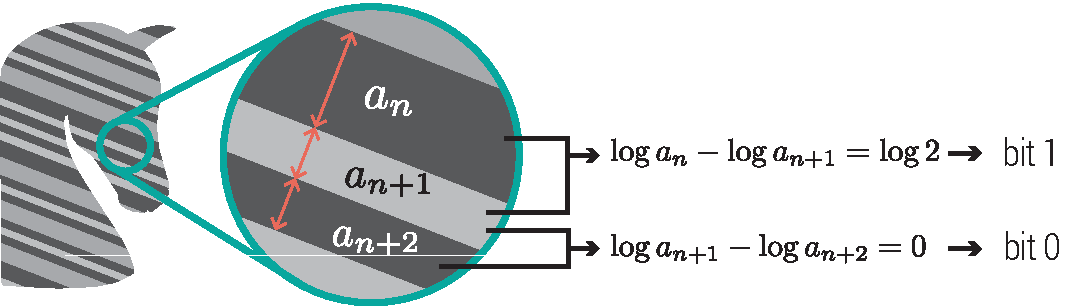
\includegraphics[width=0.85\columnwidth]{figs/ratio.pdf}
    \vspace{-2mm}
    \caption{\textbf{Encoding scheme.} Pairs of layers encode a single bit. A bitwise $0$ or $1$ can be determined by computing the ratio of adjacent layer thicknesses.
    \label{fig:ratio}}
    \vspace{-7mm}
\end{figure}

For further details regarding choice of $M$, guarantees surrounding information capacity, and encoding bitstring direction, repetition, and error correction, please refer to the full paper~\cite{Maia:2019}.

\subsection{Decoding}\label{sec:layercode_decode}

We propose a \emph{graph-based} algorithm in order to robustly tackle the challenges
associated with decoding the proposed scheme from image pixels of complex geometries. 
This is achieved by first constructing a graph to 
represent the potentially fragmented layer structure.
We treat each coding layer region, which may
not include an entire layer, as a graph node. 
Two nodes are connected if they are from
different but neighboring layers.

\begin{figure}[t]
    \centering
    \vspace{-7mm}
	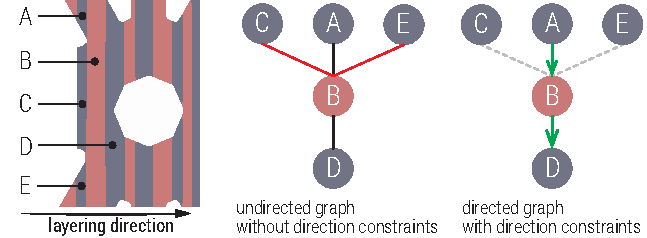
\includegraphics[width=0.80\linewidth]{figs/graph.pdf}
        \vspace{-1mm}
        \caption{\textbf{Graph construction and traversal. } 
        (left) Pixel regions are identified (A-E) through flood filling.
        (middle) Nodes are connected to form a graph if their regions are adjacent to each other.
        Since layers are added along the printing direction, it makes no
        sense to traverse backwards along a direction whilst
        decoding. Thus, A$\to$B$\to$C would not produce a valid bit string,
        while A$\to$B$\to$D is reasonable (right).
	\label{fig:directed_graph}}
    \vspace{-4mm}
\end{figure}

\paragraph{Graph Construction}\label{sec:graph_construction}
Through a flood-fill process, we identify individual pixel regions where all pixels
share a category as a preprocessing step.
Each region is represented as a graph node, and two nodes are connected if their regions are
adjacent to each other (\ref{fig:directed_graph}-a,b).

Next, we associate every graph edge $e$ with two quantities, a 2D vector
$\bm{v}$ in image space and a binary label $r$.
Consider an edge $e$ that connects nodes $A$ and $B$.
% Its vector $\bm{v}$ represents the
% general direction along which we can move from the image region $A$ to the region $B$.
% As will become clear shortly, this direction will guide us
% in traversing the graph without getting trapped in a loop. 
% To compute $\bm{v}$, we
% first identify boundary pixels in each region. These are the pixels within $\delta$ pixels
% away from another region ($\delta=3$ in practice).
At each boundary pixel, we estimate a boundary \emph{normal} direction as the direction along
which we can enter into a different region by moving the shortest distance.
$\bm{v}$ is then defined as the average normal direction over all boundary pixels between
region $A$ and region $B$.
When computing the average, we use the normal direction $\bm{n}_p$ for pixel $p$ in region $A$.
% and the opposite normal direction $-\bm{n}_p$ for $p$ in $B$.
Thus, the average direction $\bm{v}$ is in fact associated to the \emph{directed edge} from
$A$ to $B$, and for clarity we denote it as $\bm{v}_{A\to B}$. 
% The direction for the opposite edge is just $\bm{v}_{B\to A}=-\bm{v}_{B\to A}$. %% (see \todo{FIG}).


The binary label $r$ is associated to the undirected edge, and is denoted
as $r_{A\leftrightarrow B}$ for clarity. We compute $r_{A\leftrightarrow B}$ as follows.
First, from each boundary pixel $p$ between $A$ and $B$, we estimate the layer thickness
$h_A(p)$ of the region $A$ by first finding the shortest image-plane 
vector $\bm{d}_\textrm{m}$ between $p$ and another region 
that is not $A$ or $B$ but connected to $A$.
$h_A(p)$ is then set to be the length of $\bm{d}_\textrm{m}$ projected on the normal direction $\bm{n}_p$ 
% (see \figref{farbranch}).
Symmetrically, from $p$, we also estimate the layer thickness $h_B(p)$ of $B$ using a
similar step.
Then, pixel $p$ contributes a vote for $r_{A\leftrightarrow B}$.
It votes for label ``0" if $|\log h_A(p) - \log h_B(p)|< \frac{1}{2}\log M$
(i.e., closer to 0), indicating the second case in eq.~\ref{eq:decode}
and suggesting a bit ``0" encoded between $A$ and $B$.
On the other hand, if $|\log h_A(p) - \log h_B(p)|\ge \frac{1}{2}\log M$,
it votes for label ``1'', suggesting the first case in eq.~\ref{eq:decode} and hence a bit ``1''.
The final label $r_{A\leftrightarrow B}$ is taken as the majority vote over all boundary pixels.

At first glance, assigning the label $r_{A\leftrightarrow B}$ requires a prior knowledge
of $M$, which is not known from the image.
Fortunately, our coding scheme presented in \ref{sec:layercode_encode} enables an easy and robust way of estimating
$\log M$. In the above process, we collect all
$|\log h_A(p) - \log h_B(p)|$ values for all boundary pixels on the image.
From~\ref{eq:decode}, we know that these values are expected to be either $\log M$ or 0, although
we do not know what $M$ is. If we think of each $|\log h_A(p) - \log h_B(p)|$ value
as a random variable, these random variables must be generated through a
mixture of two Gaussians (in 1D):
one is centered at 0, and another center (i.e., $\log M$)
is unknown but can be estimated using the maximum likelihood estimation~\cite{nasrabadi2007pattern}.


\paragraph{Decoding through Graph Traversal}\label{sec:graph_traversal}
% We now decode the bit string by traversing the graph.
% Our traversal repeatedly starts from each node in the set $\mathcal{S}$,
% and moves to the next node through a depth-first search (DFS).
We now decode the bit string by traversing the graph node-by-node in a depth-first manner.
Because the object is always 3D printed in a layer-by-layer fashion, we must
avoid looping back to earlier layers during the traversal.
To this end, the direction vector, $\bm{v}$, associated to each edge is helpful.
As illustrated in~\ref{fig:directed_graph}-c, consider a traversal that
reaches a node $B$ from a node $A$. In the DFS, we visit the next node $D$, only
when the moving direction from $A$ to $B$ is approximately consistent with
the moving direction from $B$ to $D$. In other words, we require
$\bm{v}_{A\to B}\cdot \bm{v}_{B\to D} \ge \Delta$ ($\Delta=0.35$ in all our examples).

This graph traversal process generates many paths and thus many bit strings.
Some of them might be erroneous due to image noise. But collectively, they are robust.
Therefore, we finalize the bit string by taking a bit-wise majority vote over all decoded bit strings.

For further remarks that improve the robustness and efficiency of decoding we defer the reader to
the original work~\cite{Maia:2019}.

\section{Evaluation}\label{sec:layercode_eval}

To validate the performance of our coding algorithm thoroughly, we must test our
algorithm on a large diversity of shapes.
In large part thanks to the ease and faithfulness generated by a photorealistic renderer,
we are able to sidestep practical concerns required to 
develop such a validating dataset through the use of synthetic examples.
A glimpse of the tested shapes is shown in Figure~\ref{fig:thingi10k}. 
This evaluation over such a virtual dataset is justified by several considerations:

\begin{enumerate}[itemsep=1pt,leftmargin=12pt,label=\roman{*}.]%,label=\alph{*}.]
\item \textit{Cost and time.}
    In terms of both cost and time, it is unaffordable to 3D print all the
    shapes in the dataset. 3D printing of a single object is usually an
    hour-long process, barring failures.
    Virtual rendering of 3D printed objects, on the other hand, can be finished in 
    a short time, and the resulting images are photorealistic.
\item \textit{Feasibility.} 
For many complex shapes that we use in this evaluation, it is hard, if not
impossible, to fabricate them via current commodity 3D printers.  But 3D printing
technology is constantly and rapidly improving. Therefore, it is desirable to
test our algorithm on those complex shapes to prepare for the future.
\item \textit{Thoroughness.}
    In a virtual environment, we can test our algorithm using a large number of 
    objects viewed from many camera angles. Thoroughly testing over all these variances 
    provides us statistical insights which in turn guide our use of LayerCode tags in practice.
    This thoroughness is made possible only through simulated experiments.
\end{enumerate}


\subsection{Dataset}

We tested our algorithm over a set of shape meshes from the Thingi10k dataset~\cite{Thingi10K}.
The testing shapes are selected through the following ``printability'' criteria: 
1) They must be watertight 2-manifolds (i.e., no self-intersections), and 
2) consist of a single connected component.
3) They should also have consistent surface normals without degenerate faces.

Following these criteria, we obtain \textbf{\ft}meshes.
Each of these meshes is processed to embed a LayerCode tag indicating the
mesh's database ID. When we encode the tag (using the procedure discussed previously),
the printing direction is chosen to be the longest dimension of the mesh, and 
the baseline layer thickness $h$ is set to repeat the tag three times.
The output of the encoding step is a shape with two sets of coding layers ready for rendering. 
Each type of layer is assigned a different material color (i.e., red and blue).
We then use the physics-based renderer Mitsuba~\cite{Mitsuba} to 
generate a photorealistic image from a given camera angle.

To understand how the view angles affect the decoding,
we uniformly sample 30 viewing directions on a sphere co-centered with the object.
All the view directions are guaranteed far from the printing direction, 
since looking along the printing direction unlikely displays the entire barcode.
Figure~\ref{fig:thingi10k} shows $18$ representative shapes and the rendered images from 
multiple view angles.
The image from each view is the only input to the decoding algorithm,
and thus each view is decoded independently.

\section{Experiments \& Results}\label{sec:layercode_exp}

\paragraph{Camera angle dependency}
Because of the surface curvature and local occlusions, from certain camera angles
the coding layers are better seen. A natural question is what camera angles are more suitable
for decoding the tag. Figure~\ref{fig:decoding_probability} reports our experiment results,
suggesting that view directions just north or south of the equator 
appear statistically the most promising for decoding tags.
% This is somewhat counter-intuitive, 
% as one might expect the directions at equator to be the most promising. 

% Our hypothesis is that these slightly titled view angles allow the coding layers to be
% viewed by avoiding more occlusions introduced by bulges at one end or the center 
% of the shape. For example, the bust in \ref{fig:decoding_probability}-top
% has its head and shoulders protrude from its center axis, making decoding hard
% from above but much easier from below.

\begin{figure}[t]
    \centering
    \vspace{-4mm}
    \includegraphics[width=0.63\linewidth]{figs/viewingAngleMap.pdf}
    \vspace{-2mm}
    \caption{
    \textbf{The decoding success rate} of each view direction is color-mapped to a sphere, whose equatorial plane is perpendicular to the printing direction. This mapping is unrolled in the Mercator projection, with representative views shown (on top) for a few points of interest.
    \label{fig:decoding_probability}}
    \vspace{-2mm}
\end{figure}


Figure~\ref{fig:viewsPerMeshSorted}
shows that some shapes can accommodate a wider range of view angles than others
for successful decoding.  For example, one shape is readable from all
30 views, whereas 44 other shapes are not decodable at all
(which account for only $0.9\%$ of the shapes in the dataset).  
On average, for any given shape, its tag is readable from $51\%$ of the viewing
directions sampled. Overall, $78.0\%$ of the shapes can be decoded in 10 views, 
$49.5\%$ can be decoded in 15 directions, 
and $21.7\%$ can succeed in 20 directions.

\begin{figure}[h]
    \centering
    \vspace{-2mm}
    \includegraphics[width=0.75\linewidth]{figs/cdfPlot_99.pdf}
    \vspace{-3mm}
    \caption{ 
    We plot the distribution of all \ft tested shapes with respect to the number of view angles from which they can be decoded successfully.
    99.6\% of the shapes can be decoded from at least one sampled view direction.
    \label{fig:viewsPerMeshSorted}}
    \vspace{-7mm}
\end{figure}


% \paragraph{Timings}
% Decoding time varies from seconds and up to $5$ minutes, depending on
% specific shapes and view angles.
% % Timing for decoding each view varies greatly from shape to shape and view to view.
% % Most attempts decoded in seconds to tens of seconds, with some shapes requiring minutes.
% %  Slicing the shape varies greatly with number of triangles, usually takes seconds.
% %  Similarly, rendering time  also depends on complexity of the shapes, i.e. number of triangles.
% Image resolution impacts decoding time, since the decoding algorithm
% involves many image processing operations.
% Our experiments use a fixed resolution $2048\times 2048$px in all rendered images,
% on par with modern smartphone cameras.
% % and windowing around the regions performing
% % operations on stencils.  
% Another contributing factor is the complexity of the graph
% constructed in the decoding step.
% %  Consequently, the number of individual regions
% %  detected, of any label, impacts performance as this results in more nodes and
% %  edges in the graph representation, each of which must be visited repeatedly for
% %  decoding.  
% Simpler shapes, curvy or flat, lead to smaller number of graph nodes, 
% and thus are faster to decode.
% %the dual representation of the image.
% %\todo{ range of nodes in the graph}
% On the other hand, holes or occlusions tend to split coding layers on the image plane 
% into separate nodes and result in a larger graph. Thus, shapes with many holes and fine
% structures take longer to decode.


\paragraph{Lower bound of $h$.}
% In \ref{sec:layercode_encode}, we derive the upper bound of $h$ from Lemma~\ref{lem1}. 
A smaller $h$ allows the object to host more copies of the tag. But if 
$h$ is too small, the coding layers will become hardly discernible on the image.
In an experiment, we progressively reduce $h$ and encode only a single copy
of an ID in the object. In this process, we keep the camera angle and image resolution
unchanged, and check at what $h$ value the decoding would fail.
Not surprisingly, the lower bound of $h$ depends on the object shape. 
Figure~\ref{fig:different_resolution} reports the results.

\begin{figure}[H]
    \centering
    \vspace{-2mm}
    \includegraphics[width=0.9\linewidth]{figs/hTestFig2.pdf}
    \vspace{-2mm}
    \caption{ \textbf{Lower bound of $h$.}
    % The decoding becomes challenging if the coding layers are made too thin.
    Here we show the smallest baseline layer thickness $h$ still readable under different views for shapes normalized to 10cm in length along the printing direction.
    \label{fig:different_resolution}}
    \vspace{-2.5mm}
\end{figure}



\chapter{Neural Snooping}\label{snoop}
\vspace{-9mm}

The graphics processing unit (GPU) is a favored vehicle for executing a neural network. 
GPUs allow difficult and sizable jobs to be treated faster, 
and have been used extensively in state of the art machine learning
pipelines across both academic and commercial settings.
The use of GPUs is motivated by the need to tune
neural network applications meticulously for each task, since designs
that can robustly resolve queries end up in high demand.
As the commercial value of accurate and performant machine learning models increases,
so too does the demand to protect neural architectures as confidential investments.
This requires a careful look at the GPU.
% We explore the vulnerability of neural networks deployed as
% black boxes across GPUs through electromagnetic side channels.

% The network reconstruction is possible due to the
% modular layer sequence in which deep neural networks are evaluated.
% -
% Cast as a graph traversal problem, we are able to piece together
% a networks architecture by examining local layer pairs against a dataset.

We apply our methodology to explore the vulnerability of neural networks deployed as
black boxes across accelerated hardware through electromagnetic side channels.
We simulate a large number of queries across diverse neural architectures
and gather side channel measurements with a cheap induction sensor.
Examining the collected signals, we discover local patterns associated with
individual computational steps, that taken together form the layers and blocks
that define neural networks.
We distill graphs from these observations that match the topology of network models
and extraction of layer-specific attributes.
By optimizing over these graphs and deducing crucial parameters,
we exploit a robust side-channel signal
that is able to generalize across both networks and hardware.
We demonstrate the potential accuracy of this side channel attack
in recovering the details required for a broad range of 
network architectures and attack scenarios.

\vspace{-2mm}
\paragraph{Objective}

% We wish to know whether each layer component's evaluation
We wish to know the extent to which networks
produce an identifiable magnetic signature, 
from which layer topology, width, function type, 
and sequence order can be inferred.
Our primary focus centers on using an electromagnetic side channel to 
reverse engineer neural architectures and their defining layer parameters.
The networks in question may be of arbitrary size and depth, and involve
combinations of fully connected, convolutional, and recurrent layers,
along with a medley of interspersed activation, normalization, and pooling
layers.
Together these layers span the basic components used to assemble most
state of the art networks and account for models used across a variety of 
machine learning 
applications~\cite{he2016vision,xu2017security,teufl2010nlp,kober2013robotics,Simonyan2014vgg,krizhevsky2012imagenet}. 
% Furthermore, there are no restrictions on the types of variables involved in the
% network, suggesting our method is type agnostic and can support
% binary, integer, or real-valued models equally. 

\vspace{-3mm}
\section{Method}\label{sec:snoop_method}

We examine the magnetic flux emanating from
a graphics processing unit's 
power cable, as acquired by a cheap \$3 induction sensor, 
and find that this signal betrays the detailed topology and
hyperparameters of a black-box neural network model. 

\begin{figure*}[ht]
    \centering
    % \vspace{-1mm}
    \includegraphics[width=0.98\textwidth]{figs/setup2-same-height.pdf}
    % \vspace{-2mm}
    \caption{ \textbf{Sensing setup.} Placement of the magnetic induction sensor on the power cord works regardless of the GPU model, providing a common weak-spot to enable current-based magnetic side-channel attacks.}
    \label{fig:physicalSensor}
    \vspace{-2mm}
\end{figure*}

To reconstruct the black-box network's structure from the acquired signal, we propose a two-step approach.
First, we estimate the network topology, such as the number and types of layers, 
and types of activation functions,
using a suitably trained neural network classifier. 
Then, for each layer, we estimate its hyperparameters 
using another set of deep neural network (DNN) models.
The individually estimated hyperparameters are then jointly optimized by solving an 
integer programming problem to enforce consistency between the layers.
We demonstrate the potential accuracy of this side-channel attack in recovering 
the details for a wide range of networks, including large, 
deep networks such as ResNet101~\cite{he2016vision}.
We further apply this recovery approach to demonstrate black-box adversarial transfer attacks.

% \subsection{Signal Analysis \& Network Reconstruction}\label{sec:snoop_method}

% We prepare for the attack by training several \emph{recovery} DNN models. 
% % We refer to training before the attack as \emph{pre}training.
% After the attacker launches a single batch query (whose input and output 
% values are irrelevant), we recover structure from the acquired signal in two stages:
% \Li topology and \Lii hyperparameters.
% To recover topology, a pretrained DNN model associates a \emph{step} to 
% every signal \emph{sample}. 
% This per-sample classification partitions the signal into segments corresponding to steps. 
% We estimate hyperparameters for each \emph{individual} segment in isolation, using a step-specific pretrained DNN model, and resolve inconsistencies  between consecutive segments using an integer program.
% The pretraining of our recovery DNN models is hardware-specific, 
% and good recovery requires data gathered from similar hardware. 

\vspace{-2mm}
\subsection{Topology Recovery}\label{sec:topo}

Since neural models function to process input data into an output,
they can be unrolled into a directed acyclical graph of network steps.
This forms the topology of the network architecture, and is how
hardware functions to process data, since layer inputs
depend on the output of other layers.
Thus, by casting individual layers as graph nodes, 
connected to other nodes by the flow of logits in the network,
we can isolate the span of signals necessary to recover a network.
Namely, looking at nodes or edges suffices to recover individual
steps of the network, which combine in sequential and semantic order
as a neural network.

Classifying steps of a model entails converting a time-series signal 
to a series of labeled operations. 
The EM signal responds only to the GPU's instantaneous performance, 
but because the GPU executes a neural network sequence, there is rich context
in both the window before and after any one segment of the signal.
Some steps are often followed by others, such as pooling operations after a series of convolutions. 
We take advantage of this bidirectional context of our signal to sequence classification problem by utilizing a recurrent neural network to classify the observed signal. 

Bidirectional Long Short-Term Memory (BiLSTM) networks are well-suited 
for processing time-series signals~\cite{graves2005bidirectional}. 
We train a two-layer BiLSTM network to classify each signal sample 
into a predicted step (see \ref{fig:signalClass}-b). 
The input to our network is a sliding window of the time-series signal,
the entirety of which is classified according to the step operations
from our simulated network architecture dataset.
We train the BiLSTM by
minimizing the standard cross-entropy loss between the predicted per-sample
labels and the ground-truth labels.

This approach proves robust at identifying the sequence of steps.
It enables all of our
experiments and all GPU's tested to
recover the layers of the target
network, including their \emph{type} 
(e.g., fully connected, convolution, recurrent, etc.), 
activation function, and any subsequent 
forms of pooling or batch normalization. 
What remains is to recover layer hyperparameters. 

\vspace{-2mm}
\subsection{Hyperparameter Estimation}\label{sec:hyper}

The number of hyperparameters that 
describe a layer type depends 
on its linear step. For instance, a CNN layer type's linear
step is described by
size, padding, kernel size, number of channels, and stride hyperparameters.
Hyperparameters within a layer must be \emph{intra-consistent}. Of the six CNN 
hyperparameters (stride, padding, dilation, input, output, and kernel size),
any one is determined by the other five.
Hyperparameters must also be \emph{inter-consistent} across consecutive layers:
the output of one layer must fit the input of the next.
A brute-force search of consistent hyperparameters easily becomes
intractable for deeper networks; we therefore first estimate
hyperparameters for each layer in isolation, 
and then jointly optimize to obtain consistency.

\vspace{-2mm}
\paragraph{Initial estimation.}
% -> feature vector, DNN
We estimate a specific hyperparameter of a specific layer type,
by pretraining a DNN. We pretrain a suite of such DNNs, 
one for each (layer type, hyperparameter) pairing. 
With the layers (and their types) recovered, we can
estimate each hyperparameter using these
pretrained (layer type, hyperparameter) recovery DNNs. 

% Each DNN is comprised of two 1024-node fully connected layers with dropout.  
These DNN accept feature vectors describing two signal
segments: the linear step and the immediately subsequent step.
The subsequent step (e.g., activation, pooling, batch
normalization) requires effort proportional to the linear step's 
output dimensions, thus its inclusion informs the estimated output dimension. 
Each segment's features involves extracting averages from
\Li partitioning the segment uniformly into $N$ windows, and
\Lii concatenating the segment's time duration.
However, there is no guarantee that this produces a valid network 
in that neighboring step estimates are consistent.

\vspace{-2mm}
\paragraph{Joint optimization.}
To enforce consistency on initial estimates we jointly optimize, 
seeking values that
\emph{best fit their initial estimates, subject to consistency constraints}.
Our optimization minimizes the convex quadratic form
\begin{equation}\label{eq:opt}
    \min_{x_i\in\mathbb{Z}^{0+}}\sum_{i\in\mathcal{X}} \left(x_i - x^*_i\right)^2 \ ,\quad
    \textrm{subject to consistency constraints,}
\end{equation}
where $\mathcal{X}$ is the set of all hyperparameters across all layers; $x^*_i$ and $x_i$
are the initial estimate and optimal value of the $i$-th hyperparameter, respectively.
The imposed consistency constraints are:
\begin{enumerate}[topsep=0mm, partopsep=0mm, leftmargin=7mm, label=(\roman*)]
    \item The output size of a layer agrees with the input size of the next layer.
    \item The input size of the first layer agrees with the input feature size.
    \item The output size of a CNN layer does not exceed its input size.
    \item The hyperparameters of a CNN layer satisfy
          \begin{equation}\label{eq:const}
              s_{\text{out}} = \left\lfloor{\frac{s_\text{in}+2\beta-\gamma(k-1)-1}{\alpha}+1}\right\rfloor,
          \end{equation}
          where $\alpha$, $\beta$, $\gamma$, and $k$ denote the layer's stride, padding, dilation, and kernel size, respectively.
    \item Heuristic constraint: the kernel size must be odd.
\end{enumerate}

Among these constraints, \textbf{(i-iii)} are linear constraints, 
which preserves the convexity of the problem.
The heuristic \Lv can be expressed as a linear constraint: 
for every kernel size parameter $k_j$, we introduce a dummy variable
$\tau_j$, and require $k_j = 2\tau_j+1$ and $\tau_j\in \mathbb{Z}^{0+}$.
Constraint \Liv, however, is troublesome, because the appearance of stride $\alpha$
and dilation $\gamma$, both of which are optimization variables, make the 
constraint nonlinear.

Since all hyperparameters are non-negative integers,
the objective must be optimized via integer programming: 
IP in general case is NP-complete~\cite{papadimitriou1998combinatorial}, 
and the nonlinear constraint \Liv does not make life easier.
Fortunately, both $\alpha$ and $\gamma$ have very narrow ranges in practice:
$\alpha$ is often set to be 1 or 2, and $\gamma$ is usually 1, and they rarely change
across all CNN layers in a network.
As a result, they can be accurately predicted by our DNN models; we therefore retain
the initial estimates and do not optimize for $\alpha$ and $\gamma$,
rendering (\ref{eq:const}) linear.
Even if DNN models could not reliably recover $\alpha$ and $\gamma$, 
one could exhaustively enumerate the few possible $\alpha$ and $\gamma$ combinations,
and solve the IP problem (\ref{eq:opt}) for each combination, and select the best recovery.

The IP problem with a quadratic objective function and linear constraints can be easily
solved, even when the number of hyperparameters is large (e.g., $>1,000$). 
In practice, we use IBM CPLEX~\cite{cplex2009v12}, a widely used IP solver.
Optimized hyperparameters remain close to the initial DNN estimates, yet differ in that
they are guaranteed to define a valid network structure.


\begin{figure}[H]
    \centering
    % \vspace{-3mm}
    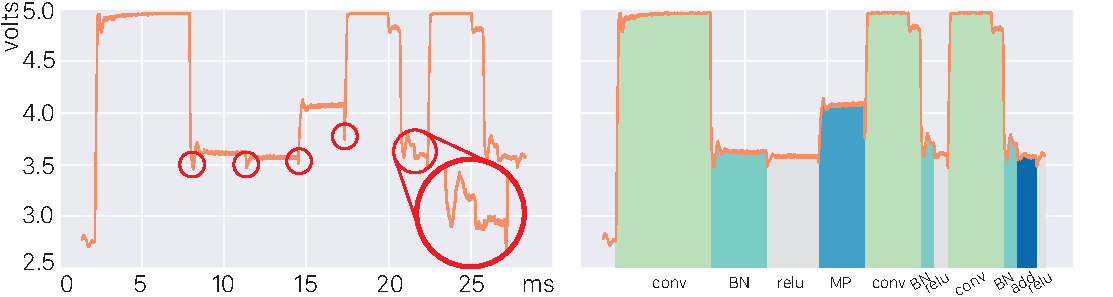
\includegraphics[width=0.90\textwidth]{figs/Fig1-3-prettier.pdf}
    \vspace{-2mm}
    \caption{\textbf{Leaked magnetic signal.} 
    (left) Our induction sensor captures a magnetic signal of 
    a CNN running on the GPU.
    % We observe strong correlation between the signal and the network steps.
    % Across two steps, t
    The GPU has to synchronize steps, resulting in 
    a sharp drop of the signal level (highlighted by selected red circles).
    (right) We can accurately classify the network steps and reconstruct the topology, as indicated by the labels under the $x$-axis. Here we highlight the signal regions associated with convolutions (conv), batch-norm (BN), Relu activations (relu), max-pooling (MP), and adding steps together (add).
    \label{fig:signalClass}}
    \vspace{-8mm}
\end{figure}

\section{Evaluation}\label{sec:snoop_eval}
% In order to benchmark the performance of 
% Some candidate metrics for evaluation are as follows:
% \begin{itemize}
%     \item distance.
%     \item accuracy.
%     \item stats.
%     \item attack.
%     \item transfer.
%     \item ablation
% \end{itemize}

\paragraph{Data capture.}
Pretraining the recovery DNN models (recall \ref{sec:snoop_method})
requires an annotated dataset with pairwise correspondence between signal and 
step types (see \ref{fig:physicalSensor}).
% FIG: example of the labelled signal
We can automatically generate an annotated signal for a given network
and specific GPU hardware, simply by executing a query (with arbitrary input values) on the 
GPU to acquire the signal. 
%The GPU is at the adversary's disposal, matching the brand/version of the
%victim, as purchased on the open market. In our experiment, we use \todo{three}
%GPU models, Nvidia GTX-960, GTX-1080, Titan V. Signals collected from each GPU are used to train
%an individual topology extraction network.
% annotation
Timestamped ground-truth GPU operations
are available by deep learning libraries (e.g., \texttt{\small torch.autograd.profiler} in PyTorch and
\texttt{\small  tf.profiler} in TensorFlow). 


\paragraph{Training Set Details.} 
The set of networks to be annotated could in principle consist \Li solely of 
randomly generated networks, on the basis that data values and ``functionality'' are irrelevant 
to us, and the training serves to recover the substeps of a layer;
or \Lii of curated networks or those found in the wild, on the basis that such 
networks are more indicative of the typical black-box. 
We construct our training set as a mixture of both approaches.

Randomly generated networks involve base steps made up of a mixture of fully-connected, recurrent, and CNN layers.
These are accompanied by $5$ different activation functions, $2$ types of pooling layers,
and a potential normalization operation.
Off the shelf networks consist of VGG and ResNet variants.
All in all we consider $500$ networks for training,
ranging from $4$ to $512$ steps per network and culminating in
$70,933$ individual steps in total.
When we construct these networks, their input image resolutions are randomly chosen from
[224$\times$224, 96$\times$96, 64$\times$64, 48$\times$48, 32$\times$32]: the highest resolution
is used in ImageNet, and lower resolutions are used in datasets such as CIFAR.

\section{Experiments \& Results}\label{sec:snoop_exp}


\begin{table}[t]
\vspace{-1mm}
\centering
\caption{Classification accuracy of network steps (Titan V) \label{tab:classify1}}
\vspace{1mm}
\scalebox{0.79}{
\begin{tabular}{l|cccc} 
\bottomrule
 Layer Type & Prec. & Rec. & F1  & \# samples \\ \hline
LSTM & .997 & .992 & .995 & 8,704 \\
Conv & .993 & .996 & .994 & 447,968  \\
Fully-connected & .901 & .796 & .846 & 10,783 \\
Add & .984 & .994 & .989 & 22,714   \\
BatchNorm & .953 &	.955 &	.954 &	47,440\\
MaxPool & .957 & .697 & .806 & 4,045 \\
AvgPool & .371 & .760 & .499 &675 \\
ReLU  & .861 & .967& .911 & 28,512\\
ELU  & .464 &.825 & .594& 2,834 \\
LeakyReLU&.732 & .578 & .646 & 9,410 \\
Sigmoid& .694 & .511 & .588& 8,744 \\
Tanh& .773& .557& .648& 4,832 \\ \hline
Weighted Avg. & \textbf{.968}& \textbf{.967} & \textbf{.966} & - \\
\toprule
\end{tabular}}
\vspace{-3mm}
\end{table}


% \paraspace
\paragraph{Topology reconstruction.}
% LSTM accuracy -> data distribution
% edit distance & L1 distance
As discussed in~\ref{sec:snoop_method}, we use a BiLSTM model
to predict the network step for each single sample.
Table~\ref{tab:classify1} reports its accuracy, measured on an Nvidia Titan V GPU. %%by Precision, Recall, and F1 score. 
There, we also break the accuracy down into measures of individual types of network steps, with an overall accuracy of \textbf{96.8\%}.
% imbalanced data; that's the real case
An interesting observation is that the training and test datasets are both
unbalanced in terms of signal samples (see last column of Table~\ref{tab:classify1}).
This is because in practice convolutional layers are computationally the most
expensive, while activation functions and pooling are lightweight.
Also, steps like average pooling are less frequently used.
While such data imbalance does reflect reality, when
we use them to train and test, most of the misclassifications occur at those
rarely used, lightweight network steps, whereas the majority of network steps
are classified correctly.

We evaluate the quality of topology reconstruction using
normalized Levenshtein edit distance that 
has been used to evaluate network structure similarity \cite{graves2006connectionist, hu2020deepsniffer}.
Here, Levenshtein distance measures the minimum number of operations---including
adding/removing network steps and altering step type---needed to 
fully rectify a recovered topology. %%%into the network's true topology. 
This distance is then normalized by the total number of steps of the target network.

% We report the detailed results in Figure~\ref{fig:distancetitanv} in the appendix. 
Among the 64 tested networks, 40 of the reconstructed
networks match precisely their targets, resulting in \emph{zero} Levenshtein distance.
The average normalized Levenshtein distance of all tested networks is \textbf{0.118},
and confirms our networks are recovered with often exact
step matches and model lengths.

To provide a sense of how the normalized Levenshtein distance is related to a network's ultimate performance, we
conduct an additional experiment to gauge reconstruction quality via classification accuracy.
We consider AlexNet (referred as model \textsf{A}) and its
five variants (refered as model \textsf{B}, \textsf{C}, \textsf{D}, and \textsf{E}, respectively).
The variants are constructed by randomly altering some of the network steps in model \textsf{A}.
The Levenshtein distances between model \textsf{A} and its variants are 1, 2, 2, 5, 
respectively, and the normalized Levenshtein distances 
are 0.05, 0.11, 0.11, 0.28 (see Fig.~\ref{fig:edit_dist}). 
We then measure the performance (i.e., standard test accuracy) of these models
on CIFAR-10. As the edit distance increases, the model's performance drops.
% \begin{figure}[t]%[14]{r}{0.5\textwidth}
% %   \vspace{-4mm}
%   \begin{center}
%     \includegraphics[width=0.47\textwidth]{figs/edit_dist_perf.pdf}
%   \end{center}
%   \vspace{-6mm}
%   \caption{Each model's classification accuracy drops as its Levenshtein distance
%       from the original model (model \textsf{A}: AlexNet) increases. \label{fig:edit_dist}}
%   \vspace{-2mm}
% \end{figure}
% % -baseline with random guess at net parameters vs optimized parameters

\paragraph{DNN hyperparameter estimation.}
Next, we report the test accuracies of our DNN models (discussed in
Ch.~\ref{sec:hyper}) for estimating hyperparameters of convolutional layers. 
Our test data here consists of 1804 convolutional layers. On average, our DNN
models have \textbf{96\%-97\%} accuracy.  The break-down accuracies for
individual hyperparameters are shown in Table~\ref{tab:dnn} of the appendix.

\begin{table}[t]
\centering
\caption{Model extraction accuracy on CIFAR-10 }\label{tab:cifarAcc}
\resizebox{\columnwidth}{!}{%
    \begin{tabular}{l|ccccc}
    \bottomrule
    {Model} & Target & Titan V & Titan X & GTX1080 & GTX960 \\ \hline
    VGG-11 & 89.03 & 89.61  & 89.63 & 88.46 & 88.3\\
    VGG-16 & 90.95 & 91.08 & 91.03 & 89.33 & 90.78\\
    AlexNet & 81.68 & 85.26 & 85.11 & 85.27 & 85.03\\
    ResNet-18 & 92.77 & 92.61 & 92.82 & 92.79 & 92.04\\
    ResNet-34 & 92.21 & 92.28 & 92.95 & 90.81 & 92.71\\
    ResNet-50 & 90.89 & 91.8 & 91.97 & 91.2 & 91.29 \\ 
    ResNet-101 & 91.58 & 91.91 & 91.85 & 91.37 & 91.72 \\ 
    \toprule
    \end{tabular}
}
\vspace{-4mm}
\end{table}

\paragraph{Reconstruction quality measured as classification accuracy.}
Ultimately, the reconstruction quality must be evaluated
by how well the reconstructed network performs in the task that the 
original network aims for. To this end, we test seven networks, including VGGs,
AlexNet, and ResNets, that have been used for CIFAR-10 classification (shown in
Table~\ref{tab:cifarAcc}). 
We treat those networks as black-box models and reconstruct them from their magnetic signals. 
We then train those reconstructed networks and compare their test accuracies with the original networks' performance.
Both the reconstructed and original networks are trained with the same training dataset for the same number of epochs. 
The results in Table~\ref{tab:cifarAcc} show that for all seven networks, including large networks (e.g., ResNet101), the reconstructed networks perform almost as well as their original versions. 

\paragraph{Transfer Attacks.}
Results of using such an approach to enable transfer attacks is deffered to Appendix~\ref{sec:transferability}.
Further findings discussing extraction and comparisons among GPUs can be found in the full text~\cite{maia2021hear}. 

\chapter{Data-Driven Hair Contact}\label{plan}
% \vspace{-9mm}
Modern hair simulation pipelines are largely throttled by their handling
of inter-strand contact. 
Accurate collision resolution between rods is
computationally expensive at scale and virtually prohibitive at large time
steps. 
The overall difficulty stems from time required to converge
on a solution to collision handling when treating large intertwined contact networks.
It is often necessary to approximate the contact handling in order
to maintain simulation progress. 
Concessions may involve adopting
a simplified contact model, curtailing the number of contacts treated, 
or limiting the time allotted towards contact resolution 
(often by capping the number of solver iterations permitted for friction handling). 
The are no guarantees
on the accuracy or convergence of the resulting contact update that
shapes each timestep of most practically sized examples.
Yet, even after surrendering accuracy, contact remains a bottleneck.
A technique for efficient large scale hair contact resolution
that addresses these shortcomings is therefore highly desirable.

We propose to continue the partnership developed between 
simulated examples and graph formulations
in order to tackle the challenges
surrounding efficiently simulating hair contact.
We will generate strand-strand contact resolution data
to pair with input collision configurations
by running a baseline hair simulation on desired examples.
Inspecting these samples we discover time-varying contact clusters
that form spatially, and their properties that inform the contact solve.
We translate these contact clusters into graphs that can be used
to train a machine learning model to infer post-solve degrees of freedom
from contact configurations.
We propose to utilize these graphs in conjunction with aggregated simulation
data to train an efficient approximate hair contact model that can be used
to exhibit large scale simulations.

\paragraph{Objective}
We are motivated to introduce a data-driven alternative that 
can expedite contact for hair simulations.
% Large scale hair contact simulations are
% troublesome and avoided due to their laboriousness to shape, 
% along with their size and time complexity.
% The overall difficulty stems from time required to converge
% on a solution to collision handling when treating large intertwined contact networks.
% , preventing creative iteration on assets. 
% Given results free of any visual artifacts, with quality assurances, or bound to
% any sort of physical principle, the added costs might prove worthwhile. 
% However, in light of the concessions already made and accepted,
% we believe it warranted to make 
However, data-driven approximations face two concerns when
applied to hair contact.
% These approximations 
% However, applying machine learning to hair contact raises two concerns. 
Firstly, elastic rods do not map naturally to existing network architectures
or model reduction techniques.
Secondly, the space of contact configurations we aim to approximate grows combinatorially.
We seek a result free of visual artifacts and flexible enough
to work with various strand models.
Any method is acceptable so long as it can
achieve similar results and reduce the costs incurred by the simulation.

% \vspace{-3mm}
\section{Method}\label{sec:hair}
We propose to train a data-driven contact resolution model based on slow albeit
accurate collision solves, so that the data used to guide our model is physically principled.
This allows us to leverage existing discrete elastic rod simulations 
that we wish to emulate with the ability to generate labeled datasets as needed.
The simulated input configurations and output collision resolutions 
generated are used to inform a neural network, 
making us the first to bridge physics-based elastic rod simulations with machine learning.

We propose to address both the structuring and constraining of
our data pairs through the use of Graph Neural
Networks~\cite{battaglia2018graphnetssummary, chang2016compositional, li2019learning, li2018propagation,  pfaff2021learning, sanchezgonzalez2018inferencecontrol, sanchezgonzalez2020learning, scarselli2009graphnets}.
We reformulate the data generated by mapping contact clusters of strands onto a graph structure.
% We take advantage of the recently growing sub-field in machine learning involving
% Graph Networks and their applications
% .
We propose a novel interpretation of dynamic piece-wise linear elastic curves in 3D as embeddings held in nodes and edges of a graph network.
Elements in the graph network are combined with machine learning algorithms
to process latent embeddings and to communicate across the graph which includes contact edges.
This transformation sidesteps the overwhelming complexity of data introduced by simulating
free curves in space with possibly varying degrees of freedom and contact stencils.
This framework allows us to moderate any exponential or combinatorial expansion of our dataset,
and constrains our efforts to solve local operators on the proposed graph. 
The resulting simulation targets foremost the improvement in efficiency of collision
resolution while remaining visually plausible. 

% \vspace{5mm}
\section{Contributions}\label{sec:hair_contributions}
Our proposed approach features the following contributions:
\begin{itemize}
    \item Fast large scale simulations trained from small scenes
    \item Stable results free of artifacts not present in training
    \item First to combine hair contact with machine learning
    \begin{itemize}
        \item A novel Graph Network processing formulation and application 
        % \item A novel Graph Network processing framework and structure 
    \end{itemize}
    \item Flexibility to replace any black box strand contact resolution scheme
    \item Model and parameter agnostic, working for straight and curly strands
\end{itemize}

% \vspace{-3mm}
\section{Setup}\label{sec:hair_exp}
The nonlinear number of collisions and changing contact bodies poses a challenge
to training a neural model which requires consistently shaped inputs.
Penetrating objects may be composed of different degrees of freedom and shapes,
making a fully connected multi-layer perceptron or convolutional network difficult
to assemble.
The elements in contact also change as collisions appear and are resolved throughout the simulation,
with no spatial-temporal coherence.
In order to manage variable sized inputs pertaining to contact clusters and strands
that change in the number of primitives involved, 
we take advantage of Graph Neural Networks.

Hair strands are formed of vertices connected by edges, and these
edges come into contact with other strands at their corresponding edges 
(i.e. edge-edge collision detection).
Therefore, rather than directly translating hair vertices and strand edges
to graph nodes and edges, we stand to benefit from viewing the \emph{dual} of
our rod structure.

We map the material edges of each strand to graph nodes.
Consequently, we connect these nodes with graph edges that represent the
internal material vertices and edges of each strand.
This enables us to treat interactions between edges, i.e. contacts,
in simulation space by connecting nodes with an edge in our graph formulation.
We categorize these volatile connections as contact edges, and together
with the nodes and internal-vertex edges they form the \hn.

\begin{figure}[H]
    \centering
    \includegraphics[width=0.95\linewidth]{figs/dualStrand.png}
    \caption{\textbf{Dual Strand.}
    We map elastic rods to a neural-amenable graph of their dual representation 
    by converting simulation edges to GraphNet nodes and connecting them with graph edges.
    \label{fig:dual_strand}}
\end{figure}


This inverted approach has several advantages. Firstly, contacts
between strands can be simply connected via a conventional edge between nodes
in the \hn, avoiding the redundancies and intricacies associated with relating
interacting edges in the primal picture.
Furthermore, discrete elastic rods exhibit twist and bending modes that are
only present at internal vertices of the strand.
Twisting and bending can be thought of as deviations to material frames
present on strand edges, and so a \hn~framework more naturally captures these
features.

Once constructed, we convert the features hosted by our 
\hn~by using the encoder-processor-decoder framework adopted by previous 
GraphNet simulation frameworks \cite{pfaff2021learning, sanchezgonzalez2020learning,sanchezgonzalez2018inferencecontrol}.
The first step converts features into an in-place latent embedding on the graph.
Next, we process our graph to relate information across adjacent and incident
graph elements (e.g. inform nodes with incident edges).
Lastly, we decode the graph back to physical quantities for use in our simulation.
In a force or contact-only based formulation, we may decode contact edges to retrieve
impulses.
If velocities are the desired output than we convert graph nodes and material edges
into the vectors of similar degrees of freedom that indicate changes to velocities
for each strand or vertex.

\begin{figure}[H]
    \centering
    \vspace{-2mm}
    \includegraphics[width=0.8\linewidth]{figs/dualContact.png}
    % \vspace{-3mm}
    \caption{\textbf{Three strands in contact.}
    Strands in contact (left) naturally form \hn s (right), where edge-edge collisions are easily  represented.
    \label{fig:dual_contact}}
    % \vspace{-5mm}
\end{figure}

\paragraph{Data Aggregation}

We take our data from the readily available and popularly used 
friction and impulse formulation of hair contact provided by discrete elastic rods.
This approach has traditionally been shown at scale
\cite{adonis14,gilles20} and suffers from 
the common contact handling bottlenecks we aim to address.
Other penalty-based variants \cite{Fei2017wetHair,li2020codimensional} may also
be used.

Training from an entirely simulated examples allows us to benefit
through principles of \emph{Direct Policy Learning}.
Rather than relying on a predetermined or constrained dataset, we instead
have an interactive demonstrator by means of our physically based target environment.
This expert oracle can be used to provide feedback on predicted 
rollout trajectories and demonstrations; 
and means we can gather new data and evolve the training dataset.

This form of \emph{Imitation learning} proves particularly fruitful given
the configuration of our simulation state across timesteps are not
independent and identically distributed from one another.
The output of one timestep (influenced by an inference) will color the input
to the next timestep.
Therefore any approximation error may lead us towards
an unfamiliar input space, and this error will accumulate as we strive to predict
from only the familiar that the network used for training.

Consequently, rather than anticipating all the data necessary for training,
it is easier for an ‘expert’ to demonstrate the target.
By utilizing the oracle to tame a possibly diverging input space,
errors neither accumulate and the agent avoids places the expert never visited.

To apply this approach, we start with 
(1) a \hn~trained on initial principled hair contact demonstrations. 
Then, we execute the following loop until we converge. 
In each iteration, we (2) collect trajectories by solving contacts 
via a \hn~(which we obtained in the previous iteration) 
and using to simulate the strands at each timestep. 
Then, for every inference, 
we (3) collect ground-truth output from the oracle 
(what would have he done in the same configuration). 
Finally, we (1) train a new \hn~policy using this feedback.

% Should add an algorithm here
\vspace{-3mm}
\section{Evaluation}

% A description of at least one initial result that is mature enough to be able to be written up for submission to a conference. Perhaps the straight hair test results.

% Next steps needed for submission.

The desired output of a hair contact pipeline is the efficient and accurate modeling
of strand-strand behavior.
% Current discrete elastic rod contact resolution pipelines rely on expensive
% iterative methods that become impractical to solve as the number of collisions increases.
We will show that by using \hn s we are able to reduce the cost of collision resolution
in hair simulations without introducing visual artifacts.
Our approach will be the first to combine strand collision resolution with
data-driven methods, and stands to benefit from the limitless data generation that
our base simulation provides.
If successful, we will not only introduce an avenue for faster large scale hair simulations,
but also pave the way for future data driven explorations relating to hair, thin structures, 
and other physics-based phenomena.

\begin{figure}[H]
    \centering
    \includegraphics[width=0.4\linewidth]{figs/hairball.png}
    \caption{\textbf{Hairball.}
    We aim to approximate grooms generated by state-of-the-art hair simulations~\cite{adonis14}
    at a fraction of the computational cost.
    \label{fig:hairball}}
\end{figure}


We are motivated by early successes in replacing contact solves with inferred approximations.
Through a mixture of \hn~and careful data aggregation, 
we have been able to simulate piles of strands coming into stable resting contact. 
We next seek to evaluate the robustness of our method to larger scale examples.
We aim to explore larger hairball examples (see Fig.~\ref{fig:hairball}) and plan to show how a 
small but representative contact scenario can inform a groom several orders of magnitude higher.
Once a stable hairball featuring thousands of strands can be demonstrated, we will
aggregate timing comparisons in order to submit our findings.


\chapter{Timeline}\label{sec:hair_plan}

Our proposed methodology calls for utilizing datasets 
of synthetic data to learn realistic behavioral models via graph algorithms. 
Simulated examples more easily provide access to labeled and controlled behaviors and interactions.
Graph formulations then constrain the space of digital features by
simplifying efforts to operations on nodes and edges of the formulated graph.

We propose to validate our methodology by studying 
its implications on additive manufacturing and computer vision objectives (Ch.~\ref{layercodes}), 
physical side channel attacks on modern GPUs of black-box neural architectures (Ch.~\ref{snoop}), 
and resolving bottlenecks in state-of-the-art strand-strand contact simulations (Ch.~\ref{plan}).
We aim to show that, compared to alternative methods, graph-based 
handling of data driven models outperforms existing works 
in terms of robustness and quality guarantees.

The timeline for completing the proposed dissertation is as follows:
\begin{todolist}
    \item[\done] LayerCodes - Fall 2019
    \item[\done] Neural Snooping - Fall 2021
    \item Thesis Proposal - Winter 2021/2022
    \item Data-Driven Hair Contact Submission - Spring 2022
    \item Thesis Writing - Spring 2022
    \item Thesis Defense - Summer 2022
\end{todolist}
Thus I plan to defend my thesis by the end of this calendar school year.

\chapter{References}\label{references}
\printbibliography[heading=none]

\vspace{-20mm}
\appendix
% \vspace{-10mm}
\chapter{\vspace{-8mm}Supplemental Findings}

\begin{figure}[H]
    \centering
    \vspace{-16mm}
    \includegraphics[width=0.75\linewidth]{figs/all_sims.pdf}
    % \vspace{-3mm}
    \caption{
    \textbf{Complex shapes.}
    A peek into the diversity of tested shapes within our database. 
    Each view presented is correctly decoded by our graph-based algorithm, including those 
    with bumpy, shell, thin, curvy, and other challenging properties.}
    \label{fig:thingi10k}
\end{figure}

\begin{figure}[t]%[14]{r}{0.5\textwidth}
  \vspace{-4mm}
  \begin{center}
    \includegraphics[width=0.7\textwidth]{figs/edit_dist_perf.pdf}
  \end{center}
  \vspace{-6mm}
  \caption{Each model's classification accuracy drops as its Levenshtein 
  distance from the original model (model \textsf{A}: AlexNet) increases. \label{fig:edit_dist}}
  \vspace{-2mm}
\end{figure}


\begin{table}[h]
\centering
\caption{\textbf{DNN estimation accuracies.}  
Using the 1804 convolutional layers in our test dataset,
we measure the accuracies of our DNN models for estimating the
convolutional layers' hyperparameters. Here, we break the accuracies down 
into the accuracies for individual hyperparameters.
}\label{tab:dnn}
\resizebox{\columnwidth}{!}{
 \begin{tabular}{r|ccccc}
\bottomrule
           & Kernel & Stride & Padding & Image-in & Image-out \\ \hline
 Precision &0.971 &0.976 &0.965 &0.968 &0.965 \\
 Recall    &0.969 &0.975 &0.964 &0.969 &0.968 \\
 F1 Score  &0.969 &0.975 &0.962 &0.967 &0.965 \\
\toprule
 \end{tabular}
 }
\end{table}

\subsection{Transfer Attack}\label{sec:transferability}
An adversarial transfer attack attempts to design an input that tricks an unknown target model. The name 
\emph{transfer} alludes to the method of attack: The attacker builds a surrogate, an approximation (informed guess) of the unknown target model, and seeks out an input that tricks the surrogate. The attacker hopes that the exploit ``transfers'' to the actual target, i.e., that an input that tricks the surrogate also tricks the target. 
The likelihood of a successful attack increases as the surrogate better approximates the target. In a black-box setting, finding an effective surrogate is very hard~\cite{demontis2019adversarial}. 
Therefore, the attacker wishes to design a more informed surrogate. One avenue toward this is to design surrogates with topology and parameters similar to the target.

\paragraph{CIFAR-10 Dataset.}
Here we test on six networks found in the wild, 
ranging from VGGs to AlexNet to ResNets, as listed on the header row of
\ref{tab:cifar}. The table shows the percent of successful transfer 
attacks over $5,000$ attempts on the CIFAR-10 dataset.

We consider each target architecture on each of four GPUs in turn (top four rows of \ref{tab:cifar}). 
We consider each such architecture-GPU combination, in turn, as black-box target. 
Using the side channel exploit, we reconstruct the target's structure to 
obtain a surrogate architecture, 
which we train on CIFAR-10 to obtain a surrogate model. 
We craft inputs that trick the surrogate, and evaluate whether those inputs also trick the target. 
Transfer attack success is defined as the percent of generated inputs (based on the surrogate) that correctly cause the trained target model to mislabel an input.
All adversarial inputs are generated via Projected Gradient Descent~\cite{madry2018towards}, using an $\epsilon$ of $0.031$ and an $\alpha$ of $0.003$ for all results.
The success rate of the transfer attacks is summarized in the upper four rows of \ref{tab:cifar}. 

To gauge the success rates of the ``side channel surrogates,'' we compare them against ``white-box surrogates.'' We build six white-box surrogates, corresponding to the six known target architectures; these white-box surrogates differ only in weights, as the surrogates are trained from scratch on CIFAR-10.
The idealized white-box surrogates serve as a benchmark for effective surrogates; refer to the success rates in the bottom six rows of \ref{tab:cifar}.

Remarkably, the ``side-channel surrogates'' offer comparable
success rates to
``white-box surrogates.'' 
The relative success of side-channel surrogates becomes more pronounced for deeper networks (ResNets), where it appears that architecture dominates sensitivity to weight values.
When the number of layers is small, as in VGG-11 and AlexNet architectures, 
the margin for error decreases, 
and more importance is given to the weights of the target. 
However, even in these cases where attack performance drops, 
the side-channel surrogates closely match the success rate 
of their white-box counterparts, 
displayed in the lower rows. 
In other words, the side-channel reconstruction effectively 
turns a black-box into a white-box attack.


\begin{table*}[t]
\centering
\vspace{-1mm}
\caption{Transfer attack results on CIFAR-10.\label{tab:cifar}}
\scalebox{0.9}{
\begin{tabular}{cl|cccccc}
\bottomrule
 & & \multicolumn{6}{c}{Target Model} \\
& & ResNet-18 & ResNet-34 & ResNet-101 & VGG-11 & VGG-16 & AlexNet \\\hline
\parbox[t]{2mm}{\multirow{11}{*}{\rotatebox[origin=c]{90}{Source Model}}} 
& GTX-960&  98.56 & 92.51 & 91.20 & 63.41 & 72.57 & 58.90\\
& GTX-1080& 97.88 & 90.86 & 86.24 & 64.69 & 55.19 & 56.83 \\
& Titan X& 98.32 & 93.45& 84.47 & 61.89 & 77.36 & 68.41\\
& Titan V& 98.48 & 93.65 & 91.27 & 64.39 & 72.77 & 60.17\\\cline{2-8}
& ResNet-18& 97.70  & 90.72 & 80.27 & 47.98 & 86.64 & 30.56\\
& ResNet-34 & 97.21 & 92.46 & 82.30 & 51.42 & 85.60 & 32.34\\
& ResNet-101 & 92.53 & 86.98 & 92.95  & 53.98 & 83.04 & 30.55\\
& VGG-11& 65.86 & 57.82 & 57.52 & 60.24 & 65.50 & 39.95\\
& VGG-16& 74.00 & 61.54 & 54.23 & 41.60 & 74.29 & 29.57\\
& AlexNet & 10.11 & 9.59& 10.19 & 11.60 & 10.42 &  62.70\\
\toprule
\end{tabular}}
\vspace{-2mm}
\end{table*}



\paragraph{MNIST Dataset.}
Similar to our analysis of CIFAR-10 transfer attacks, 
we also conduct transfer attack experiments on the MNIST dataset. 
We download four networks online, which are not commonly used.
Two of them are convolutional networks (referred as CNN1 and CNN2), and 
the other two are fully connected networks (referred as DNN1 and DNN2).
None of these networks appear in the training dataset.
We treat these networks as black-box targets, reconstruct a side-channel surrogate for each, and attack the four targets; results are shown in \ref{tab:mnist}.
As baselines, we also train white-box surrogates with the exact architecture of the four target models.


All four of our extracted networks, visible in the top row of \ref{tab:mnist} achieve high
transfer attack scores against our candidate targets.
These high scores suggest a close approximation of the target models by our reconstructed networks.
The similarity between our extracted network's transfer attack results and the results achieved
by the matching source model across the bottom four rows also indicates a strong correspondence
in the achieved architectures.
We find that even across the MNIST dataset we are able to generate a model that behaves akin to
a white-box transfer attack.
% }


\vspace{-2mm}
\begin{table}[t]
\centering
\caption{Transfer attack results on MNIST. }\label{tab:mnist}
\resizebox{0.8\columnwidth}{!}{
 \begin{tabular}{ll|cccc} 
\bottomrule
& & \multicolumn{4}{c}{Target Model} \\
& & CNN1 & CNN2 & DNN1 & DNN2 \\ \hline
\parbox[t]{2mm}{\multirow{5}{*}{\rotatebox[origin=c]{90}{Source Model}}} 
& GTX-1080 & .802 & .878 & .999 & .874 \\ 
\cline{2-6}
& CNN1 & .858 & .226 & .785 & .476 \\
& CNN2 & .395 & .884 & .354 & .354 \\
& DNN1 & .768 & .239 & .999 & .803 \\
& DNN2 & .703 & .219 & .975 & .860 \\ 
\toprule
 \end{tabular}
 }
\end{table}



\end{document}